
\chapter{Menu Volumes}\label{volumes_chapter}
\minitoc 

\section{Edit first selected volume}
This option opens the "Edit first selected volume" window.
The "Edit first selected" window can also be opened by clicking on "
\includegraphics[scale=0.7]{images/06/objects/volume_edit.png}" (see Fig. \ref{edit_volume_window}).



\begin{figure}
  \centering
  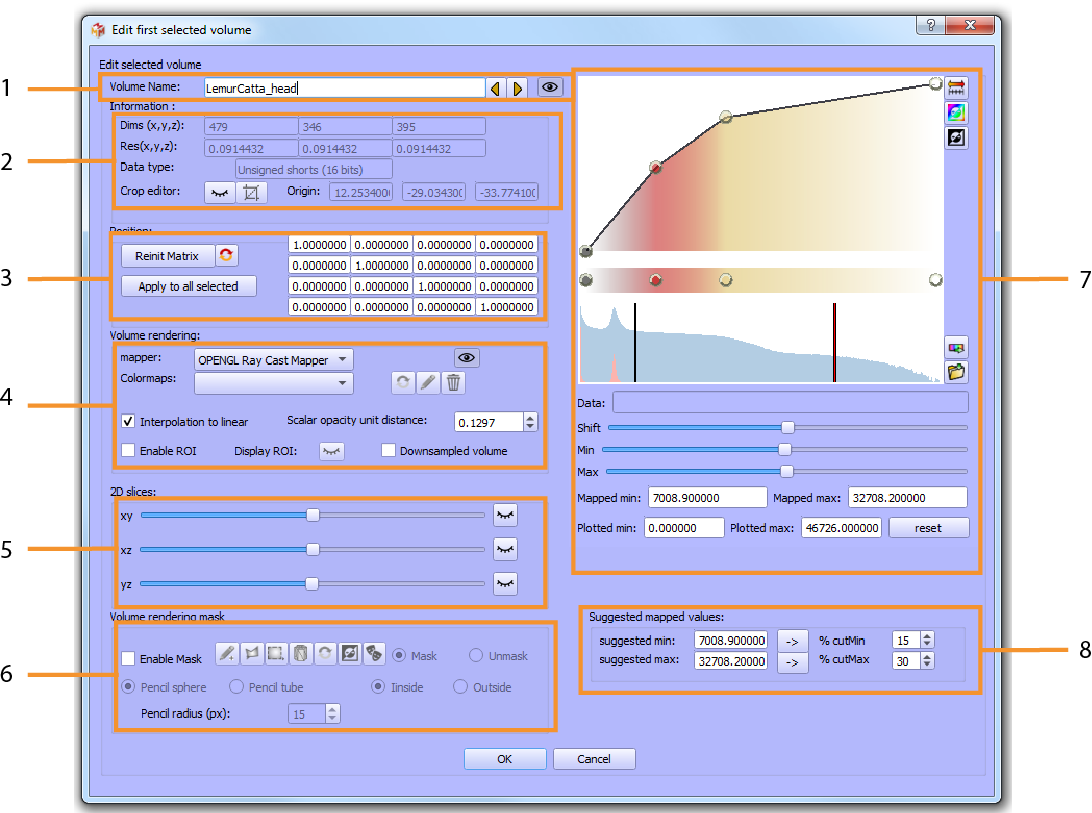
\includegraphics[scale=1]{images/14/edit_volume_window.png}
\caption{Edit first selected volume window. This window is divided in different subsections. \textbf{1)} Choose current volume to edit. Change volume name, browse through the different opened volume (arrows), and render or hide the currently activated volume rendering representation and/or 2D slices.  \textbf{2)} Information: dimensions, voxel size and data type of the currently selected volume. Crop editor: define crop region of the currently selected volume. \textbf{3)} Position matrix. Edit manually the position matrix, reinit matrix to identity, refresh matrix, and/or apply edited matrix to all selected volumes. \textbf{4)} Volume rendering. Choose mapper and colormap. Show or hide volume rendering representation. Show only a region of the currently selected volume (Enable ROI and display ROI toggles). \textbf{5)} 2D slices settings and visibility in xy, xz and yz planes. \textbf{6)} Volume rendering masking. Mask must be enabled first to activate the different masking tools : pencil sphere, pencil tube, free-form lasso, square lasso, use 3D surface to mask volume region, invert mask, and fill masked voxels.  \textbf{7)} Color map edition and histogram (orange: linear scale; blue: logarithmic scale). \textbf{8)} Map 3D volume using suggested min and suggested max values.}	
\label{edit_volume_window}
 \end{figure}

\subsection{Volume name}
\subsection{Position}
\subsection{Volume rendering}
\subsection{2D slices}
\subsection{Volume rendering mask}
\subsection{Color map edition}
\subsection{Suggested mapped values}

\section{Extract isosurface from first selected volume}

\section{Filp or swap first selected volume}
